\section{Results}
\label{sec:results}

\subsection{The committed bank reproduces}

Called on the committed ladders, the engine returns the multiplier \mAdv{} on the LiST Adverse base and \mExt{} on the LiST Extreme base at a target of 30 days, refuses the 2023 fast-run base, and reproduces the committed survival curves on the whole grid of the case design (R1 to R3). At the multiplier the survival period is 30 days and one decimal below it is 31 days, so the round trip is exact (R5), and the modelled outflow of the fast-run base in the two days of the labelled run is \svbModel{} of the deposit base (R4). The Adverse base has a survival period of \spAdv{} days and a cap of \capAdv{}, the Extreme base \spExt{} days and a cap of \capExt{}, and the fast-run base a cap of \capFast{}; the first three rows of Panel B of \cref{tab:main-results} list them.

\begin{table*}[htbp]
\centering
\small
\setlength{\tabcolsep}{3pt}
\caption{Main results. Panel A: the proposed solver and four comparators scored against the independent oracle on 20,000 instances of the seeded corpus; rates in per cent with 95\% Wilson intervals, median absolute relative error of the multiplier on solved instances, mean forward evaluations per solved instance and median time per call. Panel B: the same solver on the three committed bases of case C16 at a target of 30 days, with the survival period reached at the multiplier and just below it.}
\label{tab:main-results}
\begin{tabular}{p{2.8cm}p{2.3cm}p{2.3cm}p{2.3cm}p{1.5cm}p{1.6cm}p{1.1cm}}
\toprule
\multicolumn{7}{l}{\textit{Panel A: corpus of synthetic banks}} \\
Method & answers where refused (\%) & no answer where solved (\%) & threshold property (\%) & median $|$rel. error$|$ & evaluations & ms per call \\
\midrule
proposed solver & 0.0 (0.0 to 0.0) & 0.0 (0.0 to 0.0) & 100.0 (100.0 to 100.0) & 8.9e-08 & 15.7 & 0.29 \\
scan of the case grid & 93.5 (93.0 to 93.9) & 3.1 (2.7 to 3.4) & 0.0 (0.0 to 0.0) & 2.2e-01 & 9.7 & 1.88 \\
scan of a fine grid & 93.7 (93.3 to 94.1) & 1.4 (1.2 to 1.7) & 0.0 (0.0 to 0.0) & 1.3e-02 & 171.6 & 35.14 \\
Brent on the survival period & 13.5 (12.9 to 14.2) & 0.0 (0.0 to 0.0) & 15.7 (14.9 to 16.4) & 6.3e-02 & 15.0 & 0.30 \\
bisection without refusal & 100.0 (100.0 to 100.0) & 0.0 (0.0 to 0.0) & 99.0 (98.7 to 99.2) & 9.2e-08 & 61.4 & 2.97 \\
\bottomrule
\end{tabular}

\medskip

\begin{tabular}{p{3.0cm}p{3.0cm}p{1.4cm}p{2.3cm}p{1.8cm}p{2.3cm}}
\toprule
\multicolumn{6}{l}{\textit{Panel B: committed bases of case C16, target of 30 days}} \\
Base & base SP (days) & cap & multiplier $m^\ast$ & SP at $m^\ast$ & SP at $m^\ast-10^{-6}$ \\
\midrule
LiST Adverse & 62 & 145.2 & 2.118175 & 30 & 31 \\
LiST Extreme & 41 & 93.9 & 1.383141 & 30 & 31 \\
2023 fast run & survives (5-day horizon) & 18.4 & refused, no number & -- & -- \\
\bottomrule
\end{tabular}
\end{table*}


\begin{figure}[htbp]
\centering
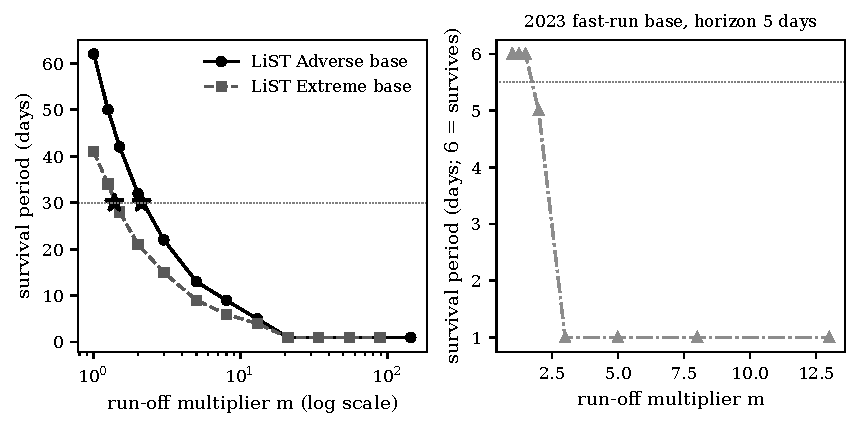
\includegraphics[width=0.98\textwidth]{sp-curve}
\caption{Survival period against the run-off multiplier on the three committed bases of case C16: the LiST Adverse and Extreme bases on the left with the thirty-day target as a dotted line and the threshold multipliers marked by stars, and the 2023 fast-run base on the right with its five-day ladder, on which a survival period of 6 stands for surviving the horizon.}
\label{fig:sp-curve}
\end{figure}

\Cref{fig:sp-curve} shows why the integer survival period is a poor object to invert. On the Adverse base it falls from \spAdv{} days at $m=1$ to 32 days at $m=2$ and 22 days at $m=3$, so the grid of the case design brackets the target between 2 and 3 and does not locate it; the solver returns \mAdv{}. On the fast-run base the curve shows that the base survives the five days up to $m=1.5$, reaches day 5 at $m=2$ and day 1 at $m=3$, so a thirty-day target is meaningless on it: no survival period under thirty days can be told from surviving the ladder, and the refusal is the correct answer rather than a failure of the solver.

The solved multiplier depends on the target as \cref{prop:threshold} says. \Cref{fig:by-target} plots it against $T$ for the two LiST bases; it is non-increasing, defined up to a target of \tMaxAdv{} days on the Adverse base and \tMaxExt{} days on the Extreme base, and refused from the survival period of the base upwards. The dotted lines are the hyperbolic rule $\mathrm{SP}(1)/T$ of \cref{prop:hyperbolic}; at 30 days it gives \hypAdv{} on the Adverse base and \hypExt{} on the Extreme base, \hypAdvErr{}\,\% and \hypExtErr{}\,\% from the solved values.

\begin{figure}[htbp]
\centering
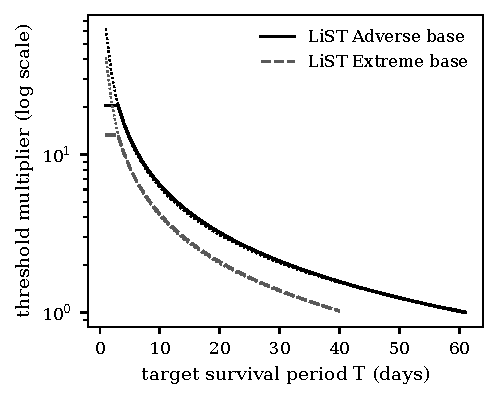
\includegraphics[width=0.6\textwidth]{by-target}
\caption{Threshold multiplier against the target survival period for the LiST Adverse and Extreme bases of case C16, on a logarithmic axis; the dotted lines are the hyperbolic rule equal to the survival period of the unscaled base divided by the target, and each curve ends at the largest target below the survival period of its base.}
\label{fig:by-target}
\end{figure}

\subsection{The corpus: solver against comparators}

The corpus has \kInst{} instances, \kSolved{} of which the oracle solves and \kRefused{} of which it refuses (\cref{tab:design}): \kHor{} because the target is not below the horizon, \kBase{} because the base already reaches it and \kUnr{} because no multiplier under the cap does.

\begin{table}[htbp]
\centering
\small
\setlength{\tabcolsep}{3pt}
\caption{Composition of the seeded corpus: 5 independent corpora of 1,000 synthetic banks, each solved at the targets of 2, 5, 10 and 30 days, counted by the outcome of the independent oracle.}
\label{tab:design}
\begin{tabular}{lr}
\toprule
Outcome of the oracle & Instances \\
\midrule
instances (banks $\times$ targets) & 20,000 \\
solved by the oracle & 8,568 \\
refused: target not below the horizon & 5,034 \\
refused: base survival period already at or below the target & 5,870 \\
refused: no multiplier under the cap reaches the target & 528 \\
solved, constant capacity and no inflow & 2,318 \\
solved, capacity on a monetisation schedule & 5,177 \\
\bottomrule
\end{tabular}
\end{table}


The engine's outcome equals the oracle's on every instance (H1: \kHOneDis{} disagreements). On the solved instances its multiplier exceeds the oracle's root by between \kHTwoMin{} and \kHTwoMax{} millionths, which is the rounding step, and every one satisfies the threshold property (H2). Panel A of \cref{tab:main-results} gives the comparison. The proposed solver answers none of the refused instances and leaves none of the solved ones without a number; its median relative error is \kPErr{}, about the rounding step, and it costs \kPEvals{} evaluations of the position on average. The scan of the case grid answers \kGFalse{}\,\% of the refused instances, because it returns the first grid point, 1, when the base already reaches the target; it finds no multiplier on \kGMiss{}\,\% of the solved ones; and its median relative error is \kGErrPc{}\,\%, with a 95th percentile of \kGErrQ{}. The finer grid cuts the median error to \kFErrPc{}\,\% at \kFEvals{} evaluations per solved instance and a median call of \kFTime{} ms against \kPTime{} ms for the solver. Brent's method on the survival period answers \kBFalse{}\,\% of the refused instances and returns a threshold on only \kBThr{}\,\% of the solved ones. The bisection without the refusal rule answers every refused instance, and returns a multiplier above the cap of the scenario on \kNBeyond{}\,\% of all instances.

\begin{figure}[htbp]
\centering
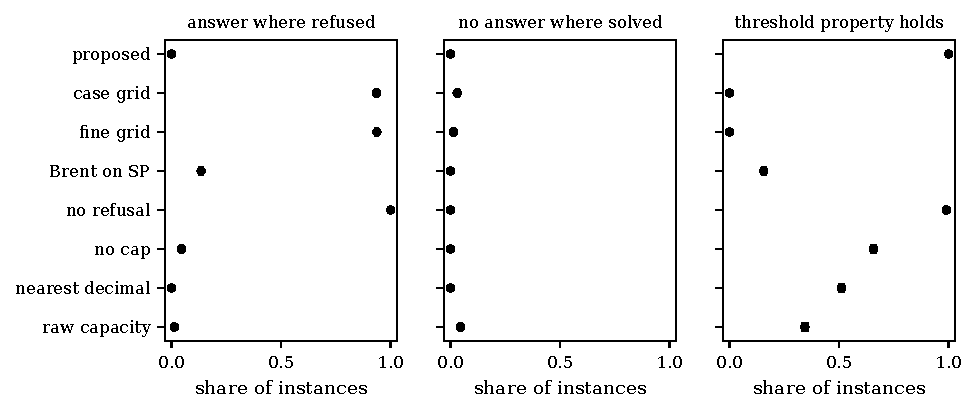
\includegraphics[width=0.98\textwidth]{methods}
\caption{Behaviour of the proposed solver and seven variants on the 20,000 instances of the corpus: from left to right the share of refused instances that are answered with a number, the share of solved instances left without an answer, and the share of solved instances whose multiplier is a threshold, each with a 95\% Wilson interval.}
\label{fig:methods}
\end{figure}

\Cref{fig:methods} shows the same three rates for all eight variants. Only the proposed solver is at 0, 0 and 1 together; the variants that remove one component differ from it in one of the three. The case grid overshoots the threshold by more than 10\% on \kHFour{}\,\% of the solved instances it answers, with a median overshoot of \kHFourMed{}\,\% and a 90th percentile of \kHFourQ{}\,\%, so H4 held. Brent's method returns a multiplier more than a millionth above the threshold on \kHFive{}\,\% of the solved instances, so H5 held: the interval on which the survival period equals the target is wide, and the root finder stops somewhere inside it.

H6 failed. On the solved instances with a constant capacity, no inflow and a finite base survival period, the multiplier $\mathrm{SP}(1)/T$ is within 10\% of the threshold on \kHSix{}\,\% of the instances, against the 80\% predicted, and the median relative error is \kHSixMed{}\,\%. \Cref{fig:scatter} shows the cause: with several segments of different rates the survival period of the unscaled run is set by the slow segments and the threshold by the fast ones, and the single-segment bounds of \cref{prop:hyperbolic} do not extend. On the committed bank the rule is within \hypAdvErr{}\,\% and \hypExtErr{}\,\%, close because one segment holds most of the deposits.

\begin{figure}[htbp]
\centering
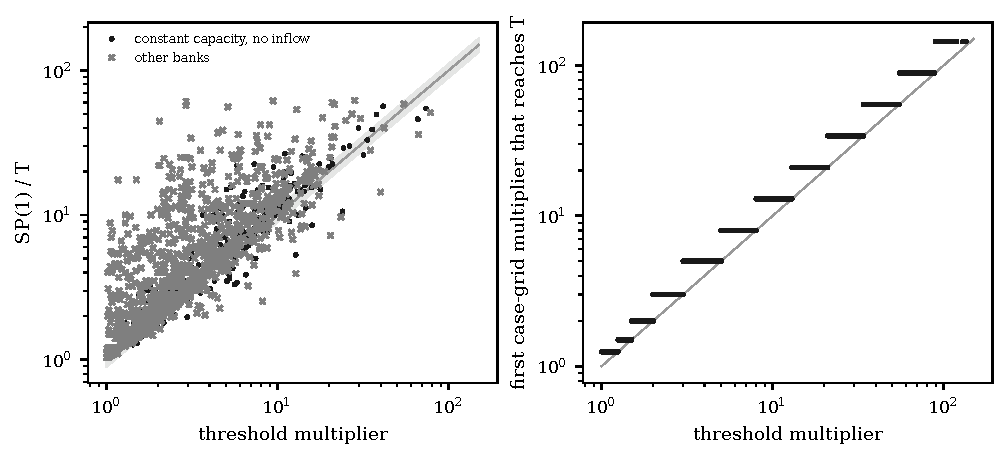
\includegraphics[width=0.98\textwidth]{scatter}
\caption{Left: the multiplier SP(1)/T against the oracle's threshold on a sample of 2,500 solved corpus instances, on logarithmic axes, with the identity line and a band of 10\%; banks with a constant capacity and no inflow are plotted as dots, the others as crosses. Right: the first multiplier of the case grid that reaches the target against the threshold, which lies above the identity line wherever the grid is coarse.}
\label{fig:scatter}
\end{figure}

\subsection{The round trip and the gap}

With a constant capacity and no inflow the survival period at the reported multiplier is exactly the target on \kHThreeMono{}\,\% of the \kFlat{} solved instances, as \cref{prop:roundtrip} states, and the sufficient condition of that proposition holds on all of them with a margin of at least \thErMarginMin{} (the outflow of day $T$ over $\delta Q_T$). With a monetisation schedule the survival period at the multiplier is below the target on \kHThreeGrow{}\,\% of the \kGrow{} solved instances, with a median gap of \kHThreeGapFifty{} days, a 90th percentile of \kHThreeGapNine{} days and a maximum of \kHThreeGapMax{} days (\cref{fig:gap}). H3 held in both clauses, the second by a wide margin. The gap is not a defect of the solver: the threshold property holds for every one of these instances. It is a property of capacity that grows, and it is the reason the method reports the survival period at the multiplier next to the multiplier.

\begin{figure}[htbp]
\centering
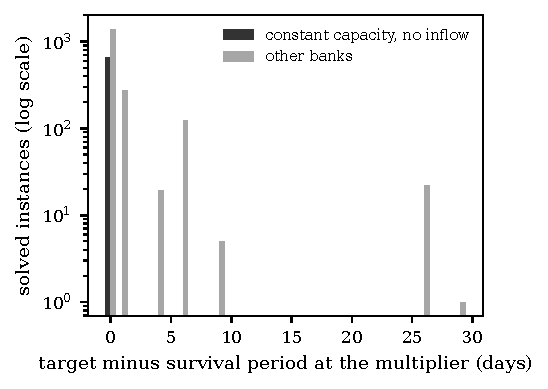
\includegraphics[width=0.6\textwidth]{gap}
\caption{Distribution of the gap between the target and the survival period at the reported multiplier over the solved corpus instances, separately for banks with a constant capacity and no inflow, where the gap is always zero, and for the other banks, where a growing capacity or an inflow can move the minimum of the window function to an earlier day.}
\label{fig:gap}
\end{figure}

On the committed fast-run base the same effect appears in a case the engine solves. With a target of 1, 2 or 3 days the multiplier is the same, \mTwo{}: the monetisation schedule releases capacity on days 1 to 3 and the survival period steps from \spBelowTwo{} days to day 1 across one decimal of the multiplier, so no multiplier gives a survival period of exactly 2 or 3. A target of 4 days is solved at \mFour{} with a survival period of 4, and a target of 5 days, equal to the horizon, is refused.

\subsection{Conventions and sensitivity}

The threshold moves with the capacity as \cref{prop:sensitivity} predicts. At the Adverse multiplier the critical day is day \dayZeroAdv{}, the elasticity of the multiplier with respect to the capacity is \elastAdv{}, and the derivative of \cref{eq:sensitivity} differs from the central difference of repeated solves by \derivRelAdv{}\,\% on the Adverse base and \derivRelExt{}\,\% on the Extreme base, within the 1\% of H7. Handing the solver the capacity schedule alone, without the inflows and the flows outside the segments, changes the Adverse multiplier from \mAdv{} to \rawAdv{} and the Extreme one from \mExt{} to \rawExt{}, \rawAdvPct{}\,\% on the Adverse base.

\begin{table}[htbp]
\centering
\small
\setlength{\tabcolsep}{3pt}
\caption{Sensitivity of the threshold multiplier at a target of 30 days to the conventions of case C16: the haircut band of 0.05, the immediate and slow monetisation schedules, the placement of the uninsured balance, and the three corners of the joint band that use the slow schedule; the last column is the survival period at the multiplier, which is the target wherever the round trip is exact and falls short of it where the slow schedule turns the threshold into a step; a refusal is stated, never a number.}
\label{tab:band}
\begin{tabular}{lrrr}
\toprule
Convention changed & Multiplier & Change (\%) & SP at $m^\ast$ \\
\midrule
\multicolumn{4}{l}{\textit{LiST Adverse base, central multiplier 2.118175}} \\
haircut low & 2.229711 & +5.3 & 30 \\
haircut high & 1.946672 & -8.1 & 30 \\
monetisation immediate & 2.118175 & +0.0 & 30 \\
monetisation slow & refused & & \\
uninsured as operational deposits & 2.796956 & +32.0 & 30 \\
uninsured as other legal entities & refused & & \\
joint: haircut low and slow monetisation & 1.063646 & -49.8 & 4 \\
joint: haircut central and slow monetisation & refused & & \\
joint: haircut high and slow monetisation & refused & & \\
\multicolumn{4}{l}{\textit{LiST Extreme base, central multiplier 1.383141}} \\
haircut low & 1.456144 & +5.3 & 30 \\
haircut high & 1.270925 & -8.1 & 30 \\
monetisation immediate & 1.383141 & +0.0 & 30 \\
monetisation slow & refused & & \\
uninsured as operational deposits & 1.936593 & +40.0 & 30 \\
uninsured as other legal entities & refused & & \\
joint: haircut low and slow monetisation & refused & & \\
joint: haircut central and slow monetisation & refused & & \\
joint: haircut high and slow monetisation & refused & & \\
\bottomrule
\end{tabular}
\end{table}


\Cref{tab:band} gives the effect of each convention. Moving every haircut by 0.05 changes the Adverse multiplier to \hcLowAdv{} (up \hcLowAdvPct{}\,\%) or \hcHighAdv{} (down \hcHighAdvPct{}\,\%). The slow monetisation schedule, which releases 25\% of the capacity on day 1 and all of it by day 10, lowers the capacity inside the window so far that the base survival period falls to \slowSpAdv{} days on the Adverse base and \slowSpExt{} days on the Extreme base, below the target of 30, and the solver refuses both. Mapping the uninsured balance to operational deposits raises the Adverse multiplier to \opAdv{} and the survival period of the base to \opSpAdv{} days. Mapping it to other legal entities, whose rate is 1 on day 1, makes the base survival period \legalSp{} day, and the solver refuses, as H9 predicted. The joint band does not keep the multiplier within 25\%: over the \jointSolvedAdv{} of nine combinations of haircut and monetisation that remain solved, the Adverse multiplier runs from \jointMinAdv{} to \jointMaxAdv{}, a deviation of \jointDevAdv{}\,\% from the central value, and H8 failed. The multiplier is stable to the haircut band alone and undefined, not unstable, under the slow schedule.

\begin{figure}[htbp]
\centering
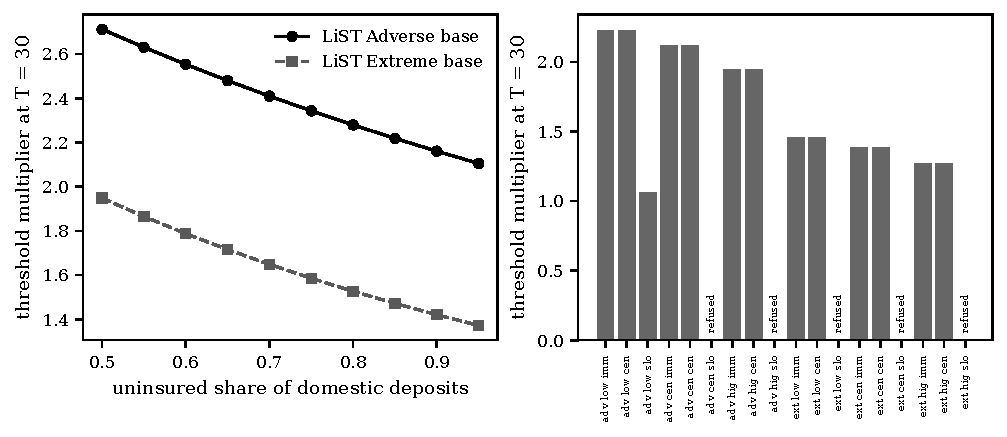
\includegraphics[width=0.98\textwidth]{band}
\caption{Threshold multiplier of the LiST Adverse and Extreme bases at a target of 30 days: on the left against the uninsured share of domestic deposits from 0.5 to 0.95, and on the right for the nine combinations of the haircut band and the immediate, central and slow monetisation schedules, with a refusal marked where the base already reaches the target.}
\label{fig:band}
\end{figure}

The multiplier also falls as the uninsured share rises (\cref{fig:band}, left): on the Adverse base it is \uninsLowAdv{} at a share of 0.5 and \uninsHighAdv{} at 0.95, since more of the deposit base sits in the segment with the faster rate and less run-off acceleration is needed to exhaust the capacity.

\subsection{The labelled run}

\begin{table}[htbp]
\centering
\small
\setlength{\tabcolsep}{3pt}
\caption{The fast-run base calibrated on the Table A.1 rows dated before 2023 and scored on the rows of the run: the modelled cumulative outflow share at the horizon of each row, its ratio to the observed share and the light of the case design (green from 0.8, amber from 0.5); rows with a horizon beyond the 5-day ladder are not scored.}
\label{tab:labelled-run}
\begin{tabular}{lccccc}
\toprule
Row & Days & Observed & Modelled & Ratio & Light \\
\midrule
SVB 2023 (scored) & 2 & 0.85 & 0.1708 & 0.201 & red \\
First Republic 2023 & 90 & 0.57 & beyond the 5-day ladder & -- & -- \\
SVB UK 2023 (scored) & 1 & 0.30 & 0.1263 & 0.421 & red \\
Credit Suisse 2023 & 90 & 0.21 & beyond the 5-day ladder & -- & -- \\
Signature 2023 (scored) & 1 & 0.20 & 0.1263 & 0.631 & amber \\
Icesave 2008 & 75 & 0.20 & beyond the 5-day ladder & -- & -- \\
Northern Rock 2007 (calibration) & 4 & 0.20 & 0.2528 & 1.264 & green \\
WaMu 2008 & 10 & 0.10 & beyond the 5-day ladder & -- & -- \\
IndyMac 2008 & 14 & 0.08 & beyond the 5-day ladder & -- & -- \\
\bottomrule
\end{tabular}
\end{table}


\Cref{tab:labelled-run} scores the fast-run base. Calibrated on the four rows dated before 2023, its rate is \rateMax{} per day, taken from the Northern Rock row; scored on the 2023 rows with horizons inside the ladder, it models \svbModel{} of the deposit base in the two days of the run against the observed 0.85, a ratio of \svbRatio{} and a red light. Against the second denominator of the case, the 140 billion dollars of outflow over the call-report deposits, which give a realised share of \depShare{}, the ratio is \depRatio{}. The two one-day rows are \ukRatio{} (red) for the sister bank in the United Kingdom, with \ukModel{} modelled against 0.30, and \sigRatio{} (amber) for the other failed bank of 2023. The in-sample row of Northern Rock is modelled at \nrModel{}, a ratio of \nrRatio{}. H10 failed: the base does not reach the amber bar at the event horizon.

The shortfall is not an artefact of the calibration rule. Replacing the maximum implied rate by the median (\rateMed{}) or the mean (\rateMean{}) lowers the ratio to \medRatio{} and \meanRatio{} (H12 held). The maximum itself rests on one row: leaving out Northern Rock leaves the maximum at \looNr{}, the rate of the WaMu row, and the other three leave-one-out fits return \rateMax{}.

\begin{figure}[htbp]
\centering
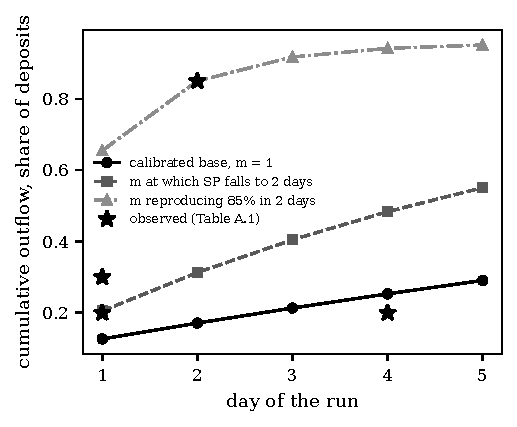
\includegraphics[width=0.6\textwidth]{labelled-run}
\caption{Modelled cumulative outflow, as a share of deposits, over the five days of the fast-run ladder at three multipliers of the calibrated rates, the calibrated base, the multiplier that brings the survival period to two days and the multiplier of the labelled run, against the observed rows of Table A.1 whose horizon lies inside the ladder, marked by stars.}
\label{fig:labelled-run}
\end{figure}

The reverse stress turns the shortfall into a distance. \Cref{fig:labelled-run} shows that the multiplier at which the modelled outflow reaches 0.85 in two days is \mSvb{}, against a cap of \capFast{} on the fast-run base, and that at this multiplier the survival period is one day. The multiplier that merely brings the survival period of the base to two days is \mTwo{}, so the multiplier of the labelled run is \ratioLab{} times larger and H11 held. In the model, the observed run lay far beyond the point at which the capacity is exhausted: a calibrated base that is red against the observation is not a base that is safe, because it takes a multiplier of \mTwo{} to exhaust its capacity. Both statements are about a synthetic bank.

\subsection{Outcome of every prediction}

\begin{table*}[htbp]
\centering
\small
\setlength{\tabcolsep}{3pt}
\caption{Reproductions and predictions with the value each one took. R1 to R5 restate values committed before the design document named them; H1 to H12 were written into a file whose modification time precedes that of the three result files (\cref{sec:experimental-design}). Three predictions failed (H6, H8, H10): the hyperbolic rule, the stability of the Adverse multiplier over the joint convention band, and the amber bar of the labelled run.}
\label{tab:hypotheses}
\begin{tabular}{lp{4.6cm}p{3.0cm}p{3.4cm}l}
\toprule
Id & Statement & Criterion & Measured & Outcome \\
\midrule
R1 & reproduction & Adverse multiplier 2.118175 & 2.118175 & reproduced \\
R2 & reproduction & Extreme multiplier 1.383141 & 1.383141 & reproduced \\
R3 & reproduction & fast run refused at 30 days & refused & reproduced \\
R4 & reproduction & modelled 2-day loss 0.17083 & 0.17083 & reproduced \\
R5 & reproduction & round trip of the threshold & SP 30, just below 31 & reproduced \\
H1 & outcome equals the oracle's & 0 disagreements & 0 of 20,000 & held \\
H2 & threshold within the rounding step & 0 to $10^{-6}$ above the root & 0.000 to 1.000 $\times10^{-6}$ & held \\
H3 & exact round trip: flat capacity; schedule & $\ge$99\%; $\ge$5\% with a gap & 100.0\%; 28.9\% & held \\
H4 & case grid overshoots by more than 10\% & $\ge$30\% of the solved instances & 75.7\% answered, 73.4\% all & held \\
H5 & Brent on SP misses the threshold & $\ge$10\% of solved & 82.6\% & held \\
H6 & SP(1)/T within 10\% of the threshold & $\ge$80\%, flat capacity & 42.7\% & failed \\
H7 & derivative equals finite difference & within 1\% & 0.0045\% & held \\
H8 & Adverse multiplier within 25\% over the band & $<$25\% & 49.8\% & failed \\
H9 & uninsured as legal entities: refusal & refused & refused & held \\
H10 & 2-day outflow reaches the amber bar & ratio $\ge$0.5 & 0.201 & failed \\
H11 & labelled multiplier $\ge2\times$ that bringing SP to 2 days & $\ge$2 & 4.58 & held \\
H12 & other calibration rules stay below amber & ratio $<$0.5 & 0.131 & held \\
\bottomrule
\end{tabular}
\end{table*}


\Cref{tab:hypotheses} lists the reproductions and predictions with the value each took. Nine of the twelve predictions held; H6, H8 and H10 failed. The failures bear on different parts of the method: the quick rule of H6 is not a substitute for the solver once several segments are present, the Adverse multiplier of H8 is not insensitive to the joint conventions, and the calibrated base of H10 does not reproduce the speed of the March 2023 run. The predictions that held are the ones that concern the solver itself, its agreement with the oracle, its threshold, its round trip and its comparison with the scans; the ones that failed concern what the committed bank and the calibrated run do. The reproductions R1 to R5 are not predictions and are not counted among the twelve.
